
目前Mesa3D的主要结构如图\ref{fig:Mesa3D}所示:


\begin{figure}[H] 
  \centering
  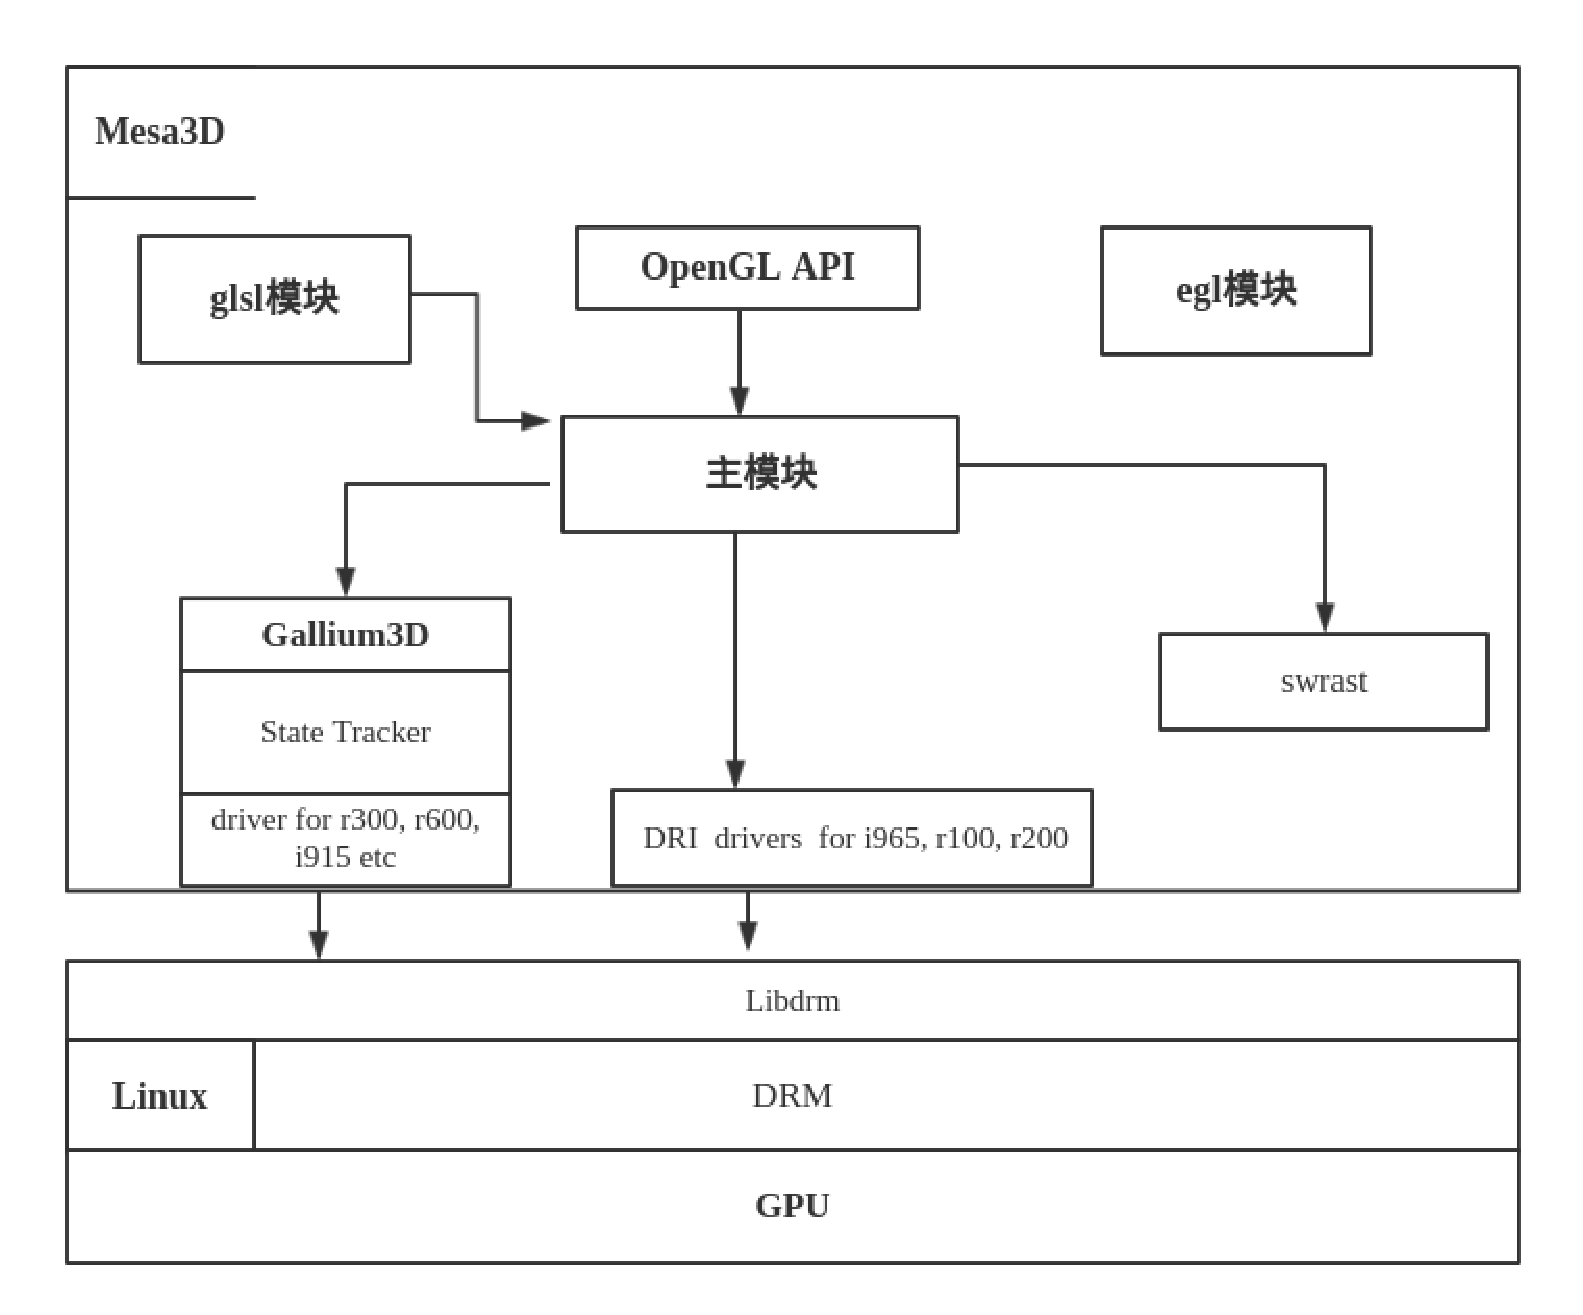
\includegraphics[width=16cm,height=12cm]{figures/chap02/Mesa3D}
  \caption{Mesa3D主要结构}
  \label{fig:Mesa3D}
\end{figure}

下面详细介绍图\ref{fig:Mesa3D}里面的几个模块:

\begin{itemize}
\item{\textbf{主模块}}: \\
Mesa3D的核心模块,它承接所有OpenGL API,并且负责vbo管理、处理glsl编译代码等工作。
\item{\textbf{glsl模块}}: \\
GLSL编译器。此模块将产生Mesa自有的IR(Intermediate Representation)。
\item{\textbf{egl模块}}: \\
EGL库实现模块。此模块是可选模块,在编译Mesa3D时候可配置是否需要。
\item{\textbf{swrast主模块}}: \\
OpenGL API渲染的软件实现模块。例如通过软件实现画点、画线、位图等。
\item{\textbf{DRI Driver for i976 等}}: \\
一些Gallium3D不支持的相关图形硬件的DRI驱动模块,比如i976、r100、r200等GPU。
\item{\textbf{Gallium3D}}: \\
Gallium3D实现模块,用来实现跨图形硬件的渲染技术。
\end{itemize}

其中主模块和Gallium3D模块是论文的研究重点所在。而Gallium3D虽然属于Mesa3D的一个组成部分,但它同样是一个开源的图形项目,它提供一套统一的API,这套API将标准的硬件特性暴露出来,通过Gallium3D将可以与统一的硬件级特性打交道,它是解决图形硬件加速问题的新方法。其主要结构如图\ref{fig:Gallium3D}所示。

\begin{figure}[H] 
  \centering
  
\includegraphics[width=10cm,height=5cm]{figures/chap02/Gallium3D}
  \caption{Mesa3D 模型结构}
  \label{fig:Gallium3D}
\end{figure}

由于Gallium3D不仅支持OpenGL也支持Direct3D等API,所以Gallium3D先是通过其内部的State Tracker模块将Mesa3D主模块的API转化为统一的State Tracker接口,然后接着根据图形硬件信息交给对应图形硬件设备驱动处理,最后调用硬件设备进行硬件加速。
